\documentclass{article}



\usepackage{fullpage}
%\usepackage{nopageno}
\usepackage{amsmath}
\usepackage{amsfonts}
\usepackage{graphicx}
\usepackage{framed}
\usepackage{xcolor}

\definecolor{dark_red}{rgb}{0.5,0.0,0.0}
\definecolor{dark_green}{rgb}{0.0,0.5,0.0}
\definecolor{dark_blue}{rgb}{0.0,0.0,0.5}

\newcommand{\dr}[1]{\textcolor{dark_red}{#1}}
\newcommand{\dg}[1]{\textcolor{dark_green}{#1}}
\newcommand{\db}[1]{\textcolor{dark_blue}{#1}}


\begin{document}

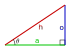
\includegraphics[width = 0.3\textwidth]{right_triangle_v2}

\begin{description}
%%%%%%%%
\item[Problem 1 (2 marks):] Given a right triangle that has a named angle of \(\theta = 65^\circ\), and an adjacent of \(a = 67.22\), compute both the opposite \(o\) and the hypotenuse \(h\) to 4 significant digits.
%%%%%%%%
\item[Problem 2 (2 marks):] Given a right triangle that has a named angle of \(\theta = 40^\circ\), and a hypotenuse of \(h = 3.500 \times 10^5\), compute both the adjacent \(a\) and the opposite \(o\) to 4 significant digits. 
%%%%%%%%
\item[Problem 3 (2 marks):] Given a right triangle that has a named angle of \(\theta = 50^\circ\), and an opposite of \(o = 9.988 \times 10^{-3}\), compute both the adjacent \(a\) and the hypotenuse \(h\) to 4 significant digits.    
%%%%%%%%
\item[Problem 4 (2 marks):] ~~~~ \\   
\begin{tabular}{cc}
\parbox{0.5\textwidth}{
In the \(x,y\) coordinate system, is a box of width \(w_x\) and height \(w_y\). The bottom left corner of the box is anchored to the origin \((0,0)\) point. Initially the box's width \(w_x\) is along the positive \(x\) axis, and the box's height \(w_y\) is along the positive \(y\) axis. The box is rotated counterclockwise by an angle of \(\theta\) with the bottom left corner still anchored to the origin point. Find the new \(x\) and \(y\) coordinates \((x',y')\) of the top right corner of the box after the rotation. {\bf Give \(x'\) and \(y'\) as expressions involving only the quantities \(w_x\), \(w_y\), and \(\theta\).} 
} & \parbox{0.4\textwidth}{
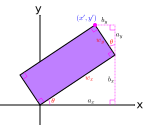
\includegraphics[width = 0.4\textwidth]{tilted_box}
}
\end{tabular}
%%%%%%%%
\item[Problem 5 (15 marks):] Fill in the table below: \\
For each empty cell, insert one of the following values or ranges: \\
\(0\), \(1\), \(-1\), \(\pm\infty\), \((0, 1)\), \((-1, 0)\), \((0, +\infty)\), \((-\infty, 0)\), \((1, +\infty)\), \((-\infty, -1)\) \\
The chosen range must be tight: the range \((0, +\infty)\) is the incorrect choice when the range is actually \((1, +\infty)\). \\
\begin{tabular}{|c||c|c||c|c||c|c|}
\hline
\(\theta\)                            & \(\cos\theta\) & \(\sin\theta\) &  \(\tan\theta\) & \(\sec\theta\) &  \(\cot\theta\) &  \(\csc\theta\) \\
\hline
\hline
\(\theta = 0\)                      &              \(1\) &               \(0\) &                \(0\) &                \(1\) &    \(\pm\infty\) &     \(\pm\infty\) \\
\hline
\(\theta \in (0, \pi/2)\)        &         \((0,1)\) &         \((0,1)\) & \((0,+\infty)\) & \((1,+\infty)\) & \((0,+\infty)\) & \((1,+\infty)\) \\
\hline
\(\theta = \pi/2\)                &               \(0\) &               \(1\) &    \(\pm\infty\) &    \(\pm\infty\) &                \(0\) &                 \(1\) \\
\hline
\(\theta \in (\pi/2, \pi)\)     &        \((-1,0)\) &        \((0,1)\) &  \((-\infty, 0)\) & \((-\infty, -1)\) & \((-\infty,0)\) & \((1,+\infty)\) \\
\hline
\(\theta = \pi\)                  &                        &                       &                         &                          &                       &                         \\
\hline
\(\theta \in (\pi, 3\pi/2)\)  &                        &                       &                         &                          &                       &                         \\
\hline
\(\theta = 3\pi/2\)             &                       &                       &                         &                          &                       &                         \\
\hline
\(\theta \in (3\pi/2, 2\pi)\) &                       &                       &                         &                          &                       &                         \\
\hline
\(\theta = 2\pi\)                &                       &                       &                         &                          &                       &                         \\
\hline
\end{tabular}
%%%%%%%%
\item[Problem 6 ({\bf bonus} 6 marks):] ~~~~ \\   
\begin{tabular}{cc}
\parbox{0.5\textwidth}{
In the image of the right, a tree with a known height of \(d = 10.00\text{m}\) is on top of a hill with an incline of \(\theta = 20^\circ\). From the bottom of the hill, the ``angular size" of the tree is \(\phi = 5^\circ\). Compute all of:
\begin{itemize}
\item \(x\), the {\bf horizontal} distance of the tree from the observer. 
\item \(y\), the altitude of the base of the tree.
\item \(z\), the distance of the base of the tree from the observer.
\end{itemize}
} & \parbox{0.4\textwidth}{
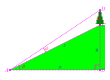
\includegraphics[width = 0.4\textwidth]{tree_on_a_hill}
}
\end{tabular}
\end{description}


\end{document}









